\subsection*{Insiemi}\label{cap:insiemi}

Un insieme (o collezione, classe, gruppo, \dots) è un concetto primitivo, ovvero è un concetto che già possediamo. Georg Cantor l'ha definito nel modo seguente: 
\begin{quote}
un insieme è una collezione di oggetti, determinati e distinti, della nostra percezione o del nostro pensiero, concepiti come un tutto unico; tali oggetti si dicono elementi dell'insieme.
\end{quote}
Mentre non è rilevante la natura degli oggetti che costituiscono l'insieme,  ciò che importa è distinguere se un dato oggetto appartenga o meno ad un insieme. Deve essere vera una delle due possibilità: il dato oggetto è un elemento dell'insieme considerato oppure non è elemento dell'insieme considerato.
Due insiemi $A$ e $B$ si dicono uguali se sono formati dagli stessi elementi, anche se disposti in ordine diverso: $A=B$. Due insiemi $A$ e $B$ si dicono diversi se non contengono gli stessi elementi:  $A \neq B$. Ad esempio, i seguenti insiemi sono uguali:
\[
\{1, 2, 3\} = \{3, 1, 2\} = \{1, 3, 2\}= \{1, 1, 1, 2, 3, 3, 3\}.
\]

Gli insiemi sono denotati da una lettera maiuscola, mentre le lettere minuscole, di solito, designano gli elementi di un insieme. 
Per esempio, un generico insieme $A$ si indica con
\[
A = \{a_1, a_2, \dots, a_n\}, \quad \text{con~} n > 0.
\]

La scrittura $a \in A$ dice che $a$ è un elemento di $A$. Per dire che  $b$ non è un elemento di $A$ si scrive $b \notin A.$

Per quegli insiemi i cui elementi soddisfano una certa proprietà che li caratterizza,
tale proprietà può essere usata per descrivere più sinteticamente l'insieme:
\[
A = \{x ~\vert~ \text{proprietà posseduta da~} x\},
\]
che si legge come ``$A$ è l'insieme degli elementi $x$ per cui è vera la proprietà indicata.'' Per esempio, per indicare l'insieme $A$ delle coppie di numeri reali $(x,y)$ che appartengono alla parabola $y = x^2 + 1$ si può scrivere:
\[
A = \{(x,y) ~\vert~ y = x^2 + 1\}.
\]

Dati due insiemi $A$ e $B$, diremo che $A$ è un \emph{sottoinsieme} di $B$ se e solo se tutti gli elementi di $A$ sono anche elementi di $B$:
\[
A \subseteq B \iff (\forall x \in A \Rightarrow x \in B).
\]
Se esiste almeno un elemento di $B$ che non appartiene ad $A$ allora diremo
che $A$ è un \emph{sottoinsieme proprio} di $B$:
\[
A \subset B \iff (A \subseteq B, \exists~ x \in B ~\vert~ x \notin A).
\]

Un altro insieme, detto \emph{insieme delle parti}, o insieme potenza, che si associa all'insieme $A$ è l'insieme di tutti i sottoinsiemi di $A$, inclusi l'insieme vuoto e $A$ stesso. Per esempio, per l'insieme $A = \{a, b, c\}$, l'insieme delle parti è:
\[
\mathcal{P}(A) = \{
\emptyset, \{a\}, \{b\}, \{c\},
 \{a, b\}, \{a, c\}, \{c, b\},
 \{a, b, c\}
\}.
\]

\subsubsection*{Operazioni tra insiemi}

Si definisce \emph{intersezione} di $A$ e $B$ l'insieme $A \cap B$ di tutti gli elementi $x$ che appartengono ad $A$ e contemporaneamente a $B$:
\[
A \cap B = \{x ~\vert~ x \in A \land x \in B\}.
\]

Si definisce \emph{unione} di $A$ e $B$ l'insieme $A \cup B$ di tutti gli elementi $x$ che appartengono ad $A$ o a $B$, cioè
\[
A \cup B = \{x ~\vert~ x \in A \lor x \in B\}.
\]

\emph{Differenza}. Si indica con $A \setminus B$ l'insieme degli elementi di $A$ che non appartengono a $B$:
\[
A \setminus B = \{x ~\vert~ x \in A \land x \notin B\}.
\]

\emph{Insieme complementare}. Nel caso che sia $B \subseteq A$, l'insieme differenza $A \setminus B$ è detto insieme complementare di $B$ in $A$ e si indica con $B^C$.

Dato un insieme $S$, una \emph{partizione} di $S$ è una collezione di sottoinsiemi di $S$, $S_1, \dots, S_k$, tali che
\[
S = S_1 \cup S_2 \cup \dots S_k
\]
e
\[
 S_i \cap S_j, \quad \text{con~} i \neq j.
\]

La relazione tra unione, intersezione e insieme complementare è data dalle leggi di DeMorgan:
\[
(A \cup B)^c = A^c \cap B^c,
\]
\[
(A \cap B)^c = A^c \cup B^c.
\]


\subsubsection*{Diagrammi di Eulero-Venn}

In molte situazioni è utile servirsi dei cosiddetti diagrammi di Eulero-Venn\footnote{I diagrammi di Venn sono così nominati in onore del matematico inglese del diciannovesimo secolo John Venn anche se Leibnitz e Eulero avevano già in precedenza utilizzato rappresentazioni simili.} per rappresentare gli insiemi e verificare le proprietà delle operazioni tra insiemi (si veda la Figura~\ref{fig:sets-venn-diagrams}). 
In tale rappresentazione, gli insiemi sono individuati da regioni del piano delimitate da una curva chiusa. 
Nel caso di insiemi finiti, è possibile evidenziare esplicitamente alcuni elementi di un insieme mediante punti, quando si possono anche evidenziare tutti gli elementi degli insiemi considerati.
\begin{figure}[h!]
  \centering
    \includegraphics[width=1.0\textwidth]{sets-venn_diagrams.pdf}
    \caption{Diagrammi di Eulero-Venn. In tutte le figure $S$ è la regione delimitata dal rettangolo, $L$ è la regione all'interno del cerchio di sinistra e $R$ è la regione all'interno del cerchio di destra. La regione evidenziata mostra l'insieme indicato sotto ciascuna figura. }
    \label{fig:sets-venn-diagrams}
\end{figure}

I diagrammi di Eulero-Venn che forniscono una dimostrazione delle leggi di DeMorgan sono forniti nella Figura~\ref{fig:demorgan}.
\begin{figure}[h!]
\centering 
   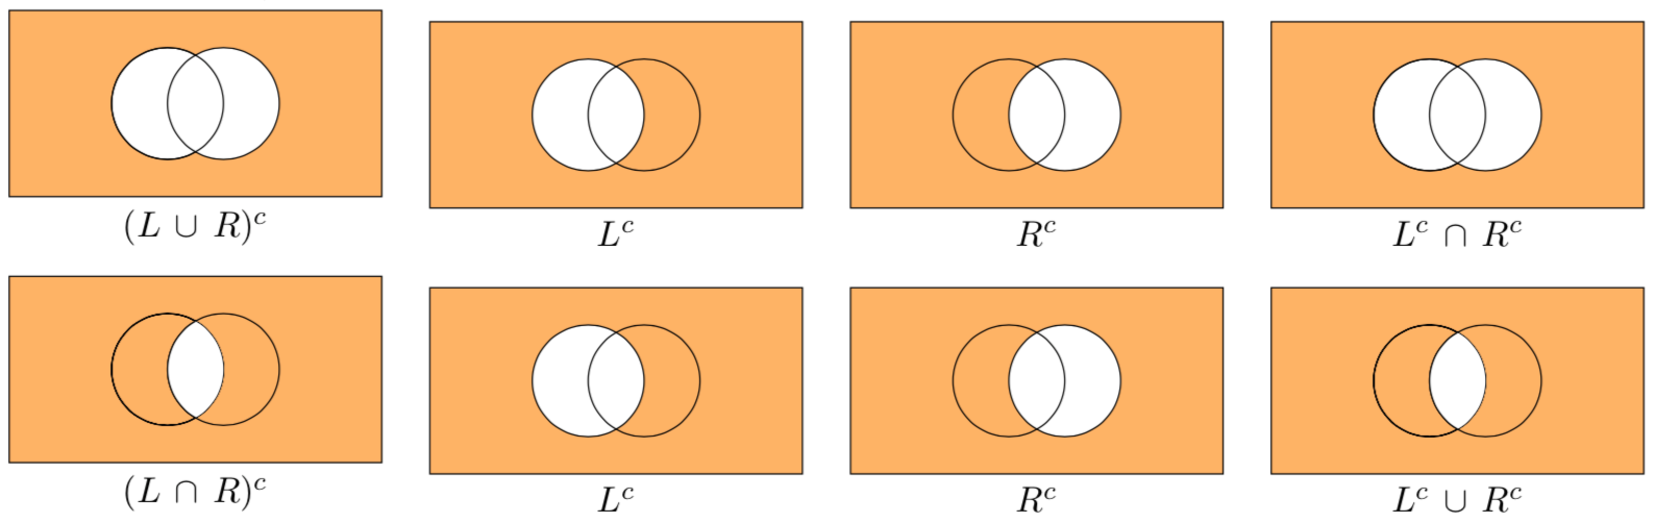
\includegraphics[width=1.0\textwidth]{demorgan.pdf}
    \caption{Dimostrazione delle leggi di DeMorgan. }
    \label{fig:demorgan}
\end{figure}

\subsubsection*{Coppie ordinate e prodotto cartesiano}
\label{sec:prod_cartesiano}

Una coppia ordinata $(x,y)$ è l'insieme i cui elementi sono $x \in A$ e $y \in B$ e nella quale $x$ è la prima componente (o prima coordinata), $y$ la seconda. 
L'insieme di tutte le coppie ordinate costruite a partire dagli insiemi $A$ e $B$ viene detto  \emph{prodotto cartesiano}:
$$A \times B = \{(x, y) ~\vert~ x \in A \land y \in B\}.$$
Ad esempio, sia $A = \{1, 2, 3\}$ e $B = \{a, b\}$. Allora,
$$
\{1, 2\} \times \{a, b, c\} = \{(1, a), (1, b), (1, c), (2, a), (2, b), (2, c)\}.
$$

\subsubsection*{Cardinalità}

Si definisce \emph{cardinalità} (o potenza) di un insieme finito il numero degli elementi dell'insieme. Viene indicata con  $\vert A\vert, \#(A)$ o $\text{c}(A)$.

%%----------------------------------------------------------------------
%\subsection*{Il principio di inclusione/esclusione}
%%----------------------------------------------------------------------
%
%Il \emph{principio di inclusione/esclusione} afferma che:
%\[
%|A \cup B| = |A| + |B| - |A \cap B|.
%\]
%Tale principio è illustrato dal diagramma di Eulero-Venn nella Figura~\ref{fig:incl-escl}.
%\begin{figure}[h]
%  \begin{center}
%    \includegraphics[width=0.5\textwidth]{incl-escl.pdf}
%    \caption{$|A|$ è il numero di punti nell'insieme $A$; lo stesso vale per $B$ e $S$. La figura mostra che $|A| + |B|$ conta due volte $|A \cap B|$, il che mostra perché $|A \cap B|$ debba essere sottratto all'interno della formula dell'inclusione/esclusione.}
%    \label{fig:incl-escl}
%     \end{center}
%\end{figure}
%
%%----------------------------------------------------------------------
%\begin{exmp}
%Supponiamo che uno psicologo segua un gruppo di pazienti. Tra essi, quattro pazienti manifestano un disturbo d'ansia, sette pazienti sono affetti da disturbo post-traumatico da stress e due pazienti manifestano sia un disturbo d'ansia sia un disturbo post-traumatico da stress. Quanti pazienti segue lo psicologo?
%\end{exmp}
%
%\begin{solu}
%Sia $A$ l'insieme di pazienti ansiosi e $P$ l'insieme dei pazienti con disturbo post-traumatico da stress. Utilizzando il principio di inclusione/esclusione, il numero cercato è:
%\[
%|A \cup P| = |A| + |P| - |A \cap P| = 4 + 7 - 2 = 9.
%\]
%\end{solu}
%%----------------------------------------------------------------------
%
%
%\begin{exmp}
%
%Se $A \subset B$, allora $\vert A \cap B\vert \leq \vert B \vert$. Le proprietà della relazione binaria di inclusione tra insiemi, che possono apparire ovvie, non  vengono però sempre rappresentate in maniera accurata nei giudizi intuitivi degli individui. \citeA{tversky1983extensional} riportano i risultati del seguente esperimento. Ad un campione di soggetti venne proposta la seguente consegna:
%\begin{quote}
%In four pages of a novel (about 2,000 words), how many words would you expect to find that have the form \_ \_ \_ \_ing (seven-letter words that end with ``ing'')?
%\end{quote}
%Ad un secondo campione, venne richiesto di stimare la frequenza delle parole aventi la forma \_ \_ \_ \_ \_n\_. Benché la seconda forma includa la prima, i soggetti si dimostrarono più propensi a giudicare la forma ``\_ \_ \_ \_ing'' come più frequente della forma ``\_ \_ \_ \_ \_n\_'' (le stime fornite dai soggetti furono di 13.4 parole in media per la prima versione e di 4.7 parole per la seconda). 
%
%Kahneman e Tversky attribuirono questo risultato all'\emph{euristica della disponibilità} secondo la quale è molto più facile recuperare in memoria parole che finiscono per ``ing'' piuttosto che parole che hanno la ``n'' in penultima posizione. \citeA{tversky1983extensional} hanno messo in evidenza come gli individui tendano ad assegnare una maggiore frequenza di occorrenza (o probabilità) agli eventi che possono essere ricordati con più facilità, rispetto agli eventi che sono più difficili da ricordare. Tuttavia, l'immagazzinamento delle informazioni in memoria non è regolato da principi statistici ma dipende invece da fattori psicologici e da limitazioni cognitive. Questo conduce gli individui a commettere sistematici errori di giudizio, come quelli che violano le proprietà della relazione binaria di inclusione tra insiemi \cite{tversky1983extensional}. 
%\end{exmp}



